Sigle identificative per i ruoli indicati nelle tabelle e nei grafici:
\begin{itemize}
    \item \textbf{RE}: Responsabile;
    \item \textbf{AM}: Amministratore;
    \item \textbf{AN}: Analista;
    \item \textbf{PT}: Progettista;
    \item \textbf{PR}: Programmatore;
    \item \textbf{VE}: Verificatore.
\end{itemize}

\rowcolors{2}{\evenRowColor}{\oddRowColor}
\renewcommand{\arraystretch}{2}
\begin{longtable}{ C{5cm} C{4cm} C{5cm} }
    \caption{Tabella di redazione}                                                                                 \\
    \rowcolor{\primaryColor}
    \textcolor{\secondaryColor}{\textbf{Ruolo}} & \textcolor{\secondaryColor}{\textbf{Costo per ora (in \euro{})}} \\ \endhead
    {\responsabile}                             & {30}                                                             \\
    {\amministratore}                           & {20}                                                             \\
    {\analista}                                 & {25}                                                             \\
    {\progettista}                              & {22}                                                             \\
    {\programmatore}                            & {15}                                                             \\
    {\verificatore}                             & {15}
\end{longtable}
\subsection{Analisi}

\subsubsection{Divisione oraria}
La seguente tabella rappresenta la distribuzione oraria dei ruoli per ogni componente del gruppo:
{

	\rowcolors{2}{\evenRowColor}{\oddRowColor}
\renewcommand{\arraystretch}{2}
\begin{longtable}[h!] { C{4cm} C{1cm} C{1cm} C{1cm} C{1cm} C{1cm} C{1cm} C{3cm}}
\caption{Tabella della divisione oraria di Analisi}	\\
\rowcolor{\primaryColor}

\textcolor{\secondaryColor}{\textbf{Membro del gruppo}} & 
\textcolor{\secondaryColor}{\textbf{RE}} & 
\textcolor{\secondaryColor}{\textbf{AM}} & 
\textcolor{\secondaryColor}{\textbf{AN}} & 
\textcolor{\secondaryColor}{\textbf{PT}} & 
\textcolor{\secondaryColor}{\textbf{PR}} & 
\textcolor{\secondaryColor}{\textbf{VE}} & 
\textcolor{\secondaryColor}{\textbf{Ore complessive}}\\	
\endhead

\AD{}                     &  - &  1 &  1 & - & - & 1 & 1 \\
\AT{}                     &  - &  - &  1 & - & - & 1 & 1 \\
\AW{}                     &  - &  - &  1 & - & - & 1 & 1 \\
\EC{}                     &  - &  1 &  1 & - & - & 1 & 1 \\
\EM{}                     &  4 &  - &  4 & - & - & 4 & 12 \\
\FP{}                     &  - &  1 &  1 & - & - & 1 & 1 \\
\GG{}                     &  4 &  - &  4 & - & - & 4 & 12 \\
\textbf{Ore totali ruolo} & X & X & X & - & - & X & X \\

\end{longtable}
}
% Responsabile color=blue, Amministratore color=yellow, Analista color=red, Progettista color=green, Programmatore color=grigetto, Verificatore color=orange  [ybar, fill=] blue, yellow, red, green, grigetto, orange
La suddivisione delle ore svolte da ciascun componente del gruppo per ogni ruolo viene rappresentata nel seguente istogramma:
\begin{center}
	\pgfplotsset{width=17cm, height=8.5cm}
	\begin{tikzpicture}
		\begin{axis}[
			ybar stacked,
			bar width=20pt,
			legend style={
				at={(0.5,-0.15)},
				anchor=north,
				legend columns=-1
			},
			symbolic x coords={Abdelwahad, Alessio, Andrea, Edoardo, Elvis, Filippo, Giovanni},
			xtick=data
		]
			\legend{Responsabile, Amministratore, Analista, Progettista, Programmatore, Verificatore}
			% Responsabile
			\addplot [ybar, fill=blue] coordinates {\ColonnaIstogramma{0}{0}{0}{0}{4}{0}{4}};
			% Amministratore
			\addplot [ybar, fill=yellow] coordinates {\ColonnaIstogramma{1}{0}{0}{1}{0}{1}{0}};
			% Analista
			\addplot [ybar, fill=red] coordinates {\ColonnaIstogramma{1}{1}{1}{1}{4}{1}{1}};
			% Progettista
			\addplot [ybar, fill=green] coordinates {\ColonnaIstogramma{0}{0}{0}{0}{0}{0}{0}};
			% Programmatore
			\addplot [ybar, fill=pink] coordinates {\ColonnaIstogramma{0}{0}{0}{0}{0}{0}{0}};
			% Verificatore
			\addplot [ybar, fill=orange] coordinates {\ColonnaIstogramma{1}{1}{1}{1}{12}{1}{12}};
		\end{axis}
	\end{tikzpicture}
\end{center}
\clearpage

\subsubsection{Costo risultante}
La seguente tabella rappresenta per ogni ruolo le ore totali investite e il corrispondente costo in euro:
{
\rowcolors{2}{\evenRowColor}{\oddRowColor}
\renewcommand{\arraystretch}{2}
\begin{longtable}{ C{3cm} C{2cm} C{4cm}}
\caption{Tabella del costo risultante di Analisi}\\
\rowcolor{\primaryColor}

\textcolor{\secondaryColor}{\textbf{Ruolo}} & 
\textcolor{\secondaryColor}{\textbf{Totale ore}} & 
\textcolor{\secondaryColor}{\textbf{Costo ruolo (in \euro{})}}\\	
\endhead

Responsabile    &  1 &  1 \\
Amministratore  &  1 &  1 \\
Analista        & 1 & 1 \\
Progettista     &   - &    - \\
Programmatore   &   - &    - \\
Verificatore    &  1 & 1 \\
\textbf{Totale} & 1 & 1 \\
		
\end{longtable}
}

\vskip 30pt %spazio verticale
La quantità di ore totali per ciascun ruolo viene rappresentata nel seguente areogramma:
\begin{center}
	\begin{tikzpicture}
		\pie[rotate = 180, color={blue, yellow, red, orange}] {
			8/Responsabile,
			16/Amministratore,
			47/Analista,
			29/Verificatore
		}
	\end{tikzpicture}
\end{center}

\newpage
\subsection{Progettazione}

\subsubsection{Divisione oraria}
La seguente tabella rappresenta la distribuzione oraria dei ruoli per ogni componente del gruppo:
\rowcolors{2}{\evenRowColor}{\oddRowColor}
\renewcommand{\arraystretch}{2}
\begin{longtable}[h!] { C{4cm} C{1cm} C{1cm} C{1cm} C{1cm} C{1cm} C{1cm} C{3cm}}
\caption{Tabella della divisione oraria della Progettazione}\\
\rowcolor{\primaryColor}

\textcolor{\secondaryColor}{\textbf{Membro del gruppo}} & 
\textcolor{\secondaryColor}{\textbf{RE}} & 
\textcolor{\secondaryColor}{\textbf{AM}} & 
\textcolor{\secondaryColor}{\textbf{AN}} & 
\textcolor{\secondaryColor}{\textbf{PT}} & 
\textcolor{\secondaryColor}{\textbf{PR}} & 
\textcolor{\secondaryColor}{\textbf{VE}} & 
\textcolor{\secondaryColor}{\textbf{Ore complessive}}\\	
\endhead
        
\AW{}                     & 10  & - & - & 8 & 8 & 5 & 32 \\
\AT{}                     & -  & 10 & - & 7 & - & 14 & 32 \\
\AD{}                     & -  & 10 & - & 7 & 9 & 9 & 33 \\
\EC{}                     & 11  & - & 4 & - & 9 & 8 & 32 \\
\EM{}                     & -  & - & 5 & 7 & 11 & 9 & 32 \\
\FP{}                     & -  & - & 6 & 10 & 10 & 7 & 33 \\
\GG{}                     & -  & - & 5 & 10 & 11 & 7 & 33 \\
\textbf{Ore totali ruolo} & 21 & 20 & 20 & 49 & 58 & 59 & 227 \\

		
\end{longtable}
La suddivisione delle ore preventivate viene rappresentata anche sottoforma del seguente istogramma:
\begin{center}
	\pgfplotsset{width=17cm, height=8.5cm}
	\begin{tikzpicture}
		\begin{axis}[
			ybar stacked,
			bar width=20pt,
			legend style={
				at={(0.5,-0.15)},
				anchor=north,
				legend columns=-1
			},
			symbolic x coords={Abdelwahad, Alessio, Andrea, Edoardo, Elvis, Filippo, Giovanni},
			xtick=data
		]
			\legend{Responsabile, Amministratore, Analista, Progettista, Programmatore, Verificatore}
			% Responsabile
			\addplot [ybar, fill=blue] coordinates {\ColonnaIstogramma{10}{0}{0}{11}{0}{0}{0}};
			% Amministratore
			\addplot [ybar, fill=yellow] coordinates {\ColonnaIstogramma{0}{10}{10}{0}{0}{0}{0}};
			% Analista
			\addplot [ybar, fill=red] coordinates {\ColonnaIstogramma{0}{0}{0}{4}{5}{6}{5}};
			% Progettista
			\addplot [ybar, fill=green] coordinates {\ColonnaIstogramma{8}{7}{7}{0}{7}{10}{10}};
			% Programmatore
			\addplot [ybar, fill=pink] coordinates {\ColonnaIstogramma{8}{0}{9}{9}{11}{10}{11}};
			% Verificatore
			\addplot [ybar, fill=orange] coordinates {\ColonnaIstogramma{5}{14}{9}{8}{9}{7}{7}};
		\end{axis}
	\end{tikzpicture}
\end{center}

\clearpage
\subsubsection{Costo risultante}
La seguente tabella rappresenta per ogni ruolo le ore totali preventivate ed il corrispondente costo in euro:
{
\rowcolors{2}{\evenRowColor}{\oddRowColor}
\renewcommand{\arraystretch}{2}
\begin{longtable}{ C{3cm} C{2cm} C{4cm}}
\caption{Tabella del costo risultante della Progettazione}\\
\rowcolor{\primaryColor}

\textcolor{\secondaryColor}{\textbf{Ruolo}} & 
\textcolor{\secondaryColor}{\textbf{Totale ore}} & 
\textcolor{\secondaryColor}{\textbf{Costo ruolo (in \euro{})}}\\	
\endhead
        
Responsabile    &  21 &  630 \\
Amministratore  &  20 &  400 \\
Analista        &  20 &  500 \\
Progettista     &  49 &  1078 \\
Programmatore   &  58 &  870 \\
Verificatore    &  59 &  885 \\
\textbf{Totale} &  227 & 4363 \\	
        	
\end{longtable}
}

\vskip 30pt %spazio verticale
La quantità di ore totali preventivate per ciascun ruolo viene rappresentata nel seguente areogramma:
\begin{center}
	\begin{tikzpicture}
		\pie[rotate = 180, color={blue, yellow, red, green, pink, orange}] {
			7/Responsabile,
			9/Amministratore,
			9/Analista,
			22/Progettista,
			27/Programmatore,
			26/Verificatore
		}
	\end{tikzpicture}
\end{center}

\subsection{Preventivo fase di Sviluppo}

\subsubsection{Divisione oraria}
La seguente tabella rappresenta la distribuzione oraria dei ruoli per ogni componente del gruppo:
{
	\rowcolors{2}{\evenRowColor}{\oddRowColor}
	\renewcommand{\arraystretch}{2}
	\begin{longtable}[h!] { C{3.5cm} C{1cm} C{1cm} C{1cm} C{1cm} C{1cm} C{1cm} C{2cm}}
	\caption{Tabella della divisione oraria fase di Sviluppo}\\
	\rowcolor{\primaryColor}
	
	\textcolor{\secondaryColor}{\textbf{Membro del gruppo}} & 
	\textcolor{\secondaryColor}{\textbf{RE}} & 
	\textcolor{\secondaryColor}{\textbf{AM}} & 
	\textcolor{\secondaryColor}{\textbf{AN}} & 
	\textcolor{\secondaryColor}{\textbf{PT}} & 
	\textcolor{\secondaryColor}{\textbf{PR}} & 
	\textcolor{\secondaryColor}{\textbf{VE}} & 
	\textcolor{\secondaryColor}{\textbf{Ore complessive}}\\	
	\endhead
	
	\AW{}                     & - & - & - & 12 & 19 & 17 & 48 \\
	\AT{}                     & 11 & - & - & 10 & 15 & 13 & 49 \\
	\AD{}                     & 10 & - & - & 7 & 18 & 14 & 49 \\
	\EC{}                     & - & - & - & 13 & 18 & 17 & 48 \\
	\EM{}                     & - & 8 & - & 10 & 19 & 11 & 48 \\
	\FP{}                     & - & 8 & - & 11 & 18 & 12 & 49 \\
	\GG{}                     & - & 8 & - & 10 & 19 & 12 & 49 \\
	\textbf{Ore totali ruolo} & 21 & 24 & - & 73 & 126 & 96 & 340\\
	
	\end{longtable}
}

% Responsabile color=blue, Amministratore color=yellow, Analista color=red, Progettista color=green, Programmatore color=grigetto, Verificatore color=orange  [ybar, fill=] blue, yellow, red, green, grigetto, orange
La suddivisione delle ore preventivate per ciascun componente del gruppo e per ogni ruolo viene rappresentata nel seguente istogramma:
\begin{center}
	\pgfplotsset{width=15.4cm, height=8.5cm}
	\begin{tikzpicture}
		\begin{axis}[
			ybar stacked,
			bar width=20pt,
			legend style={
				at={(0.5,-0.15)},
				anchor=north,
				legend columns=-1
			},
			symbolic x coords={Abdelwahad, Alessio, Andrea, Edoardo, Elvis, Filippo, Giovanni},
			xtick=data
		]
			\legend{Responsabile, Amministratore, Analista, Progettista, Programmatore, Verificatore}
			% Responsabile
			\addplot [ybar, fill=blue] coordinates {\ColonnaIstogramma{0}{11}{10}{0}{0}{0}{0}};
			% Amministratore
			\addplot [ybar, fill=yellow] coordinates {\ColonnaIstogramma{0}{0}{0}{0}{8}{8}{8}};
			% Analista
			\addplot [ybar, fill=red] coordinates {\ColonnaIstogramma{0}{0}{0}{0}{0}{0}{0}};
			% Progettista
			\addplot [ybar, fill=green] coordinates {\ColonnaIstogramma{12}{10}{7}{13}{10}{11}{10}};
			% Programmatore
			\addplot [ybar, fill=pink] coordinates {\ColonnaIstogramma{19}{15}{18}{18}{19}{18}{19}};
			% Verificatore
			\addplot [ybar, fill=orange] coordinates {\ColonnaIstogramma{17}{13}{14}{17}{11}{12}{12}};
		\end{axis}
	\end{tikzpicture}
\end{center}
\clearpage
% \subsubsection{Ore e costi degli incrementi}
% La seguente tabella rappresenta la distribuzione delle ore investite durante il periodo in cui vengono svolti gli incrementi e il corrispondente costo in euro.


% {
% \rowcolors{2}{\evenRowColor}{\oddRowColor}
% \renewcommand{\arraystretch}{1.65}
% \centering
% \begin{longtable}{ C{2.1cm} C{2.7cm} C{3cm} C{3cm} C{3.3cm} }
% \caption{Tabella del costo risultante di ogni incremento}\\
% \rowcolor{\primaryColor}
% \textcolor{\secondaryColor}{\textbf{Incremento}} & 
% \textcolor{\secondaryColor}{\textbf{Ore progettista}} &
% \textcolor{\secondaryColor}{\textbf{Ore programmatore}}&
% \textcolor{\secondaryColor}{\textbf{Ore verificatore}}&
% \textcolor{\secondaryColor}{\textbf{Costo totale incremento (in \euro{})}}\\
% \endhead


% x & x & x & x & x\\
% x & x & x & x & x\\
% x & x & x & x & x\\
% x & x & x & x & x\\
% x & x & x & x & x\\



% \end{longtable}
% }


\subsubsection{Costo risultante}
La seguente tabella rappresenta, per ruolo, le ore preventivate totali e il corrispondente costo in euro:
{
\rowcolors{2}{\evenRowColor}{\oddRowColor}
\renewcommand{\arraystretch}{2}
\begin{longtable}{ C{3cm} C{2cm} C{4cm}}
\caption{Tabella del costo risultante di Sviluppo}\\
\rowcolor{\primaryColor}

\textcolor{\secondaryColor}{\textbf{Ruolo}} & 
\textcolor{\secondaryColor}{\textbf{Totale ore}} & 
\textcolor{\secondaryColor}{\textbf{Costo ruolo (in \euro{})}}\\	
\endhead
        
Responsabile    & 21 & 630 \\
Amministratore  & 24 & 480 \\
Analista        & - & - \\
Progettista     & 73 & 1606 \\
Programmatore   & 126 & 1890 \\
Verificatore    & 96 & 1440 \\
\textbf{Totale} & 340 & 6046 \\
		
\end{longtable}
}


\vskip 30pt %spazio verticale
La quantità di ore totali preventivate per ciascun ruolo viene rappresentata nel seguente areogramma:
\begin{center}
	\begin{tikzpicture}
		\pie[rotate = 180, color={blue, yellow, green, pink, orange}] {
			6/Responsabile,
			7/Amministratore,
			22/Progettista,
			37/Programmatore,
			28/Verificatore
		}
	\end{tikzpicture}
\end{center}

\subsection{Preventivo fase di Collaudo}

\subsubsection{Divisione oraria}
La seguente tabella rappresenta la distribuzione oraria dei ruoli per ogni componente del gruppo:
{

	\rowcolors{2}{\evenRowColor}{\oddRowColor}
\renewcommand{\arraystretch}{2}
\begin{longtable}[h!] { C{4cm} C{1cm} C{1cm} C{1cm} C{1cm} C{1cm} C{1cm} C{3cm}}
\caption{Tabella della divisione oraria di Collaudo}	\\
\rowcolor{\primaryColor}

\textcolor{\secondaryColor}{\textbf{Membro del gruppo}} & 
\textcolor{\secondaryColor}{\textbf{RE}} & 
\textcolor{\secondaryColor}{\textbf{AM}} & 
\textcolor{\secondaryColor}{\textbf{AN}} & 
\textcolor{\secondaryColor}{\textbf{PT}} & 
\textcolor{\secondaryColor}{\textbf{PR}} & 
\textcolor{\secondaryColor}{\textbf{VE}} & 
\textcolor{\secondaryColor}{\textbf{Ore complessive}}\\	
\endhead

\AW{}                     &  - &  5 &  - & 10 & - & 10 & 25 \\
\AT{}                     &  - &  - &  5 & 5 & 7 & 8 & 25 \\
\AD{}                     &  - &  - &  - & - & 7 & 11 & 18 \\
\EC{}                     &  - &  10 &  - & - & 5 & 7 & 22 \\
\EM{}                     &  - &  - &  - & - & 10 & 12 & 22 \\
\FP{}                     & 10 & - &  - & - & 7 & 5 & 22 \\
\GG{}                     &  - &  - &  - & 5 & 7 & 10 & 22 \\
\textbf{Ore totali ruolo} & 10 & 15 & 5 & 20 & 43 & 63 & 156 \\

\end{longtable}
}


La suddivisione delle preventivate per ciascun componente del gruppo per ogni ruolo viene rappresentata nel seguente istogramma:
\begin{center}
	\pgfplotsset{width=17cm, height=8.5cm}
	\begin{tikzpicture}
		\begin{axis}[
			ybar stacked,
			bar width=20pt,
			legend style={
				at={(0.5,-0.15)},
				anchor=north,
				legend columns=-1
			},
			symbolic x coords={Abdelwahad, Alessio, Andrea, Edoardo, Elvis, Filippo, Giovanni},
			xtick=data
		]
			\legend{Responsabile, Amministratore, Analista, Progettista, Programmatore, Verificatore}
			% Responsabile
			\addplot [ybar, fill=blue] coordinates {\ColonnaIstogramma{0}{0}{0}{0}{0}{10}{0}};
			% Amministratore
			\addplot [ybar, fill=yellow] coordinates {\ColonnaIstogramma{5}{0}{0}{10}{0}{0}{0}};
			% Analista
			\addplot [ybar, fill=red] coordinates {\ColonnaIstogramma{0}{5}{0}{0}{0}{0}{0}};
			% Progettista
			\addplot [ybar, fill=green] coordinates {\ColonnaIstogramma{10}{5}{0}{0}{0}{0}{5}};
			% Programmatore
			\addplot [ybar, fill=pink] coordinates {\ColonnaIstogramma{0}{7}{7}{5}{10}{7}{7}};
			% Verificatore
			\addplot [ybar, fill=orange] coordinates {\ColonnaIstogramma{10}{8}{11}{7}{12}{5}{10}};
		\end{axis}
	\end{tikzpicture}
\end{center}
\clearpage
% \subsubsection{Ore e costi degli incrementi}
% La seguente tabella rappresenta la distribuzione delle ore investite durante il periodo in cui vengono svolti gli incrementi e il corrispondente costo in euro.


% {
% \rowcolors{2}{\evenRowColor}{\oddRowColor}
% \renewcommand{\arraystretch}{1.65}
% \centering
% \begin{longtable}{ C{2.1cm} C{2.7cm} C{3cm} C{3cm} C{3.3cm} }
% \caption{Tabella del costo risultante di ogni incremento}\\
% \rowcolor{\primaryColor}
% \textcolor{\secondaryColor}{\textbf{Incremento}} & 
% \textcolor{\secondaryColor}{\textbf{Ore progettista}} &
% \textcolor{\secondaryColor}{\textbf{Ore programmatore}}&
% \textcolor{\secondaryColor}{\textbf{Ore verificatore}}&
% \textcolor{\secondaryColor}{\textbf{Costo totale incremento (in \euro{})}}\\
% \endhead



% x & x & x & x & x \\
% x & x & x & x & x \\
% x & x & x & x & x \\
% x & x & x & x & x \\


% \end{longtable}
% }
\subsubsection{Costo risultante}
La seguente tabella rappresenta le ore totali investite e il corrispondente costo in euro per ogni ruolo:
{
\rowcolors{2}{\evenRowColor}{\oddRowColor}
\renewcommand{\arraystretch}{2}
\begin{longtable}{ C{3cm} C{2cm} C{4cm}}
\caption{Tabella del costo risultante di Collaudo}\\
\rowcolor{\primaryColor}

\textcolor{\secondaryColor}{\textbf{Ruolo}} & 
\textcolor{\secondaryColor}{\textbf{Totale ore}} & 
\textcolor{\secondaryColor}{\textbf{Costo ruolo (in \euro{})}}\\	
\endhead
        
Responsabile    &  10 & 300 \\
Amministratore  &  15 & 300 \\
Analista        &  5 & 125 \\
Progettista     &  20 & 440 \\
Programmatore   &  43 & 645 \\
Verificatore    &  63 & 945 \\
\textbf{Totale} & 156 & 2755 \\
	
\end{longtable}
}

\vskip 30pt %spazio verticale
La quantità di ore totali per ciascun ruolo viene rappresentata nel seguente areogramma:
\begin{center}
	\begin{tikzpicture}
		\pie[rotate = 180, color={blue, yellow, red, green, pink, orange}] {
			6/Responsabile,
			10/Amministratore,
			3/Analista,
			13/Progettista,
			27/Programmatore,
			41/Verificatore
		}
	\end{tikzpicture}
\end{center}


\subsection{Preventivo a finire completo} 
Nel preventivo riportiamo la spesa totale che il committente dovrà affrontare, derivata dal totale delle ore rendicontate e preventivate nelle fasi di Progettazione, Sviluppo,Collaudo.

\subsubsection{Divisione oraria complessiva} 
La seguente tabella rappresenta la distribuzione oraria dei ruoli per ogni componente del gruppo:
{
	\rowcolors{2}{\evenRowColor}{\oddRowColor}
\renewcommand{\arraystretch}{2}
\begin{longtable}[h!] { C{3.5cm} C{1cm} C{1cm} C{1cm} C{1cm} C{1cm} C{1cm} C{2cm}}
\caption{Tabella della divisione oraria complessiva}	\\
\rowcolor{\primaryColor}

\textcolor{\secondaryColor}{\textbf{Membro del gruppo}} & 
\textcolor{\secondaryColor}{\textbf{RE}} & 
\textcolor{\secondaryColor}{\textbf{AM}} & 
\textcolor{\secondaryColor}{\textbf{AN}} & 
\textcolor{\secondaryColor}{\textbf{PT}} & 
\textcolor{\secondaryColor}{\textbf{PR}} & 
\textcolor{\secondaryColor}{\textbf{VE}} & 
\textcolor{\secondaryColor}{\textbf{Ore complessive}}\\	
\endhead

\AW{}                     & - & 5 & 10 & 30 & 25 & 32 & 102 \\
\AT{}                     & 11 & 10 & 15 & 15 & 22 & 28 & 101 \\
\AD{}                     & 10 & 10 & - & 12 & 38 & 32 & 102 \\
\EC{}                     & 11 & 10 &  11 & 13 & 23 & 32 & 100 \\
\EM{}                     & 10 & 8  &  0 & 17 & 38 & 30 & 103 \\
\FP{}                     & 10 & 8  &  0 & 23 & 34 & 27 & 102 \\
\GG{}                     &  - & 8  & 9 & 23 & 35 & 27 & 102 \\
\textbf{Ore totali ruolo} & 52  & 59 & 45 & 133 & 215 & 208 & 712 \\
\end{longtable}
}

\subsubsection{Costo complessivo per ruolo}
Nella seguente tabella viene illustrato il monte ore risultante per ogni ruolo con il costo ad esso associato:
{
\rowcolors{2}{\evenRowColor}{\oddRowColor}
\renewcommand{\arraystretch}{2}
\begin{longtable}{ C{3cm} C{2cm} C{4cm}}
\caption{Tabella del costo complessivo per ruolo}\\
\rowcolor{\primaryColor}

\textcolor{\secondaryColor}{\textbf{Ruolo}} & 
\textcolor{\secondaryColor}{\textbf{Totale ore}} & 
\textcolor{\secondaryColor}{\textbf{Costo ruolo (in \euro{})}}\\	
\endhead
        
Responsabile   &  52 & 1560 \\
Amministratore &  59 & 1180 \\
Analista       &  29 & 725 \\
Progettista    &  142 & 3124 \\
Programmatore  &  227 & 3405 \\
Verificatore   &  218 & 3270 \\
        	
\end{longtable}
}

% La quantità di ore totali per ciascun ruolo (rendicontate e non) viene rappresentata nel seguente areogramma:
% \begin{center}
% 	\begin{tikzpicture}
% 		\pie[rotate = 180, color={blue, yellow, red, green, grigetto, orange}] {
% 			7/Responsabile, % 75/1056 circa 7%
% 			10/Amministratore, % 107/1056 circa 10%
% 			14/Analista, % 152/1056 circa 14%
% 			17/Progettista, % 181/1056 circa 17%
% 			22/Programmatore, % 227/1056 circa 22%
% 			30/Verificatore % 314/1056 circa 30%
% 		}
% 	\end{tikzpicture}
% \end{center}

Nel seguente areogramma viene rappresentata la distribuzione dei costi in percentuale sulla spesa totale da affrontare:\\
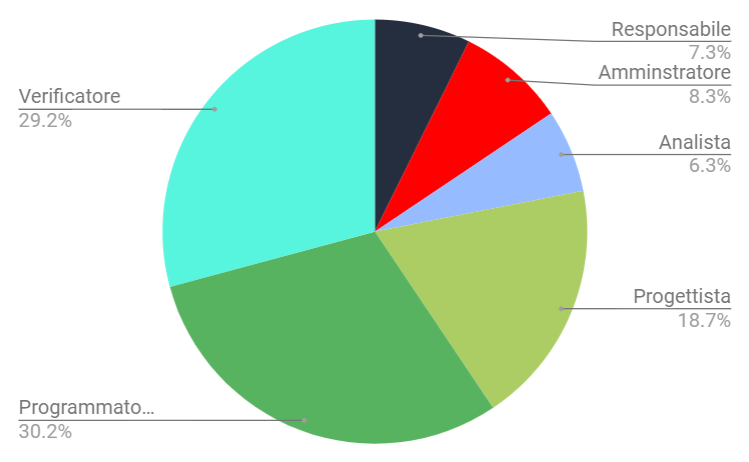
\includegraphics[width=1\textwidth]{./src/Preventivo/src/img/TortaPrevCompleto.png}
%\begin{center}
%	\begin{tikzpicture}
%		\pie[rotate = 180, color={blue, yellow, red, green, pink, orange}] {
%			7/Responsabile, % 52/723 %
%			8/Amministratore, % 59/723 %
%			4/Analista, % 29/723 %
%			20/Progettista, % 142/723 %
%			31/Programmatore, % 227/723 %
%			30/Verificatore % 218/723 %
%		}
%	\end{tikzpicture}
%\end{center}

\subsubsection{Costo complessivo}
Nella seguente tabella vengono riportati i costi complessivi delle varie fasi e infine l'importo proposto da \Gruppo{} per la realizzazione del progetto \NomeProgetto{}:\\
{
\rowcolors{2}{\evenRowColor}{\oddRowColor}
\renewcommand{\arraystretch}{2}
\begin{longtable}{ C{5cm} C{5cm}}
\caption{Tabella del costo complessivo}\\
\rowcolor{\primaryColor}

\textcolor{\secondaryColor}{\textbf{Fase}} &
\textcolor{\secondaryColor}{\textbf{Costo \glo{fase} (in \euro{})}}\\	
\endhead

Progettazione  &  4463 \\
Sviluppo & 6046  \\
Collaudo &  2755 \\
\textbf{Totale}  &  13264 \\

\end{longtable}
}
